\documentclass[11pt,twoside,titlepage,a4paper]{article}

%%%%%%%%%%%%%%%%%%%%%%%%%%%%%%%%%%%%%%%%%%%%%%%%%%%%%%%%%%%%%%%%%%%%%%%%%%%%%%%
% PAQUETES

\usepackage{xcolor} % Colores
\usepackage[xcolor]{mdframed} % Marcos
\usepackage{amsmath} % Matemáticas
\usepackage{amsfonts} % Letras caligráficas para matemáticas
\usepackage{mathtools} % Matemáticas extra
\usepackage{amsthm} % Teoremas
\usepackage{listingsutf8} % Código
\usepackage[a4paper]{geometry} % Márgenes
\usepackage{enumitem} % Opciones de personalización de listas
\usepackage{fancyhdr} % Encabezado / Pie de página
\usepackage{titlesec} % Títulos
\usepackage{pagecolor} % Colorear las portadas
\usepackage{graphicx} % Imágenes
\usepackage{hyperref} % Referencias
\usepackage{sidenotes} % Notas en el margen
\usepackage{pgfplots} % Gráficos de funciones
\usepackage{biblatex} % Bibliografía
\bibliography{InsightJournal.bib}
%%%%%%%%%%%%%%%%%%%%%%%%%%%%%%%%%%%%%%%%%%%%%%%%%%%%%%%%%%%%%%%%%%%%%%%%%%%%%%%
% COMANDOS PERSONALIZADOS

% Año o cualquier otra información para la portada
\newcommand{\fecha}{
\today
}
% Autores del documento
\newcommand{\autores}{
Blanca Cano Camarero, Manuel Gachs Ballegeer y Jose Luis Ruiz Benito
}

\newcommand{\margenimagen}{
\newgeometry{
    left=2.5cm, % Margen izquierdo
	right=5cm, % Margen derecho
	bottom=2.5cm % Margen inferior}
}
}

%%%%%%%%%%%%%%%%%%%%%%%%%%%%%%%%%%%%%%%%%%%%%%%%%%%%%%%%%%%%%%%%%%%%%%%%%%%%%%%
% TIPOGRAFÍA

\usepackage{heuristica}
\usepackage[heuristica,vvarbb,bigdelims]{newtxmath}
\usepackage[T1]{fontenc}
\renewcommand*\oldstylenums[1]{\textosf{#1}}
\usepackage[spanish]{babel}

%%%%%%%%%%%%%%%%%%%%%%%%%%%%%%%%%%%%%%%%%%%%%%%%%%%%%%%%%%%%%%%%%%%%%%%%%%%%%%%
% DEFINICIÓN DE COLORES

% COLORES DE LA ESTRUCTURA DEL DOCUMENTO
\definecolor{bg_por}{HTML}{8A0808} % Portada
\definecolor{fg_por}{HTML}{FFFFFF} % Texto de la portada
\definecolor{fg_sec}{HTML}{8A0808} % Títulos de las secciones
\definecolor{fg_ssec}{HTML}{610505} % Títulos de las subsecciones
\definecolor{fg_sssec}{HTML}{300303} % Títulos de las subsubsecciones
\definecolor{fg_head}{HTML}{610B0B} % Texto del encabezado
% COLORES PARA CÓDIGO
\definecolor{li_code}{HTML}{8A0808} % Línea a la izquierda
\definecolor{rw_code}{HTML}{610B0B} % Palabras reservadas
\definecolor{st_code}{HTML}{300303} % Cadenas de caracteres
\definecolor{cm_code}{HTML}{333333} % Comentarios
% COLORES PARA LISTAS
\definecolor{l_1}{HTML}{8A0808} % Primer símbolo
\definecolor{l_2}{HTML}{610505} % Primera indentación
\definecolor{l_3}{HTML}{300303} % Segunda indentación
\definecolor{l_4}{HTML}{000000} % Tercera indentación
% COLORES PARA MARCOS
\definecolor{li_ejs}{HTML}{8A0808} % Línea marco ejemplos
\definecolor{li_defs}{HTML}{610505} % Línea marco definiciones
\definecolor{bg_ejs}{HTML}{FFEDEE} % Fondo ejemplos
\definecolor{bg_defs}{HTML}{FFE0DF} % Fondo definiciones
% COLORES PARA REFERENCIAS
\definecolor{fg_url}{HTML}{610505} % Links


%%%%%%%%%%%%%%%%%%%%%%%%%%%%%%%%%%%%%%%%%%%%%%%%%%%%%%%%%%%%%%%%%%%%%%%%%%%%%%%
% REFERENCIAS

\hypersetup{
	pdftitle={Historia de las redes neuronales profundas}, % Título del pdf
	pdfauthor={}, % Autor del pdf
    colorlinks=true, % Referencias con color
    linkcolor=black, % Color de las referencias internas
    urlcolor=fg_url, % Color de los links
    citecolor=fg_ssec, % Color de las referencias
}
\urlstyle{same} % Links con el mismo tipo de letra

%%%%%%%%%%%%%%%%%%%%%%%%%%%%%%%%%%%%%%%%%%%%%%%%%%%%%%%%%%%%%%%%%%%%%%%%%%%%%%%
% TEOREMAS

\numberwithin{equation}{section} % Numeración de ecuaciones
% Teoremas-Lemas-Definiciones-Corolarios
\newtheoremstyle{usual} % Nombre del estilo
{} % Espacio por encima
{} % Espacio por debajo
{} % Estilo del cuerpo
{} % Indentación
{\bfseries} % Estilo de la cabecera
{} % Símbolo tras la cabecera
{ } % Espacio tras la cabecera
{\thmname{#1}\thmnumber{ #2 }\thmnote{(\textit{#3})}:} % Especificación de la cabecera
\theoremstyle{usual}
\newtheorem{theorem}{Teorema}[section] % Comando para los teoremas

%%%%%%%%%%%%%%%%%%%%%%%%%%%%%%%%%%%%%%%%%%%%%%%%%%%%%%%%%%%%%%%%%%%%%%%%%%%%%%%
% CÓDIGO

\lstset{
	basicstyle=\footnotesize\ttfamily, % Estilo del código
	inputencoding=utf8/latin1, % Codificación
	xleftmargin=1.3em, % Margen extra a la izquierda
	breaklines=true, % Romper líneas largas
	language=, % Lenguaje del código
	numbers=left, % Números de línea
	numbersep=8pt, % Separación de los números de línea
	tabsize=4, % Tamaño de los tabs
	frame=leftline, % Posición del enmarcado
	framerule=1pt, % Grosor del enmarcado
	showstringspaces=false, % Mostrar los espacios en las cadenas de caracteres
	keywordstyle=\color{rw_code}, % Estilo de las palabras reservadas
	numberstyle=\normalfont, % Estilo de los números de línea
	rulecolor=\color{li_code}, % Estilo del enmarcado
	commentstyle=\color{cm_code}, % Estilo de los comentarios
	stringstyle=\color{st_code} % Estilo de las cadenas de caracteres
}

%%%%%%%%%%%%%%%%%%%%%%%%%%%%%%%%%%%%%%%%%%%%%%%%%%%%%%%%%%%%%%%%%%%%%%%%%%%%%%%
% MÁRGENES

\geometry{
	left=2.5cm, % Margen izquierdo
	right=2.5cm, % Margen derecho
	bottom=2.5cm % Margen inferior
}

%%%%%%%%%%%%%%%%%%%%%%%%%%%%%%%%%%%%%%%%%%%%%%%%%%%%%%%%%%%%%%%%%%%%%%%%%%%%%%%
% LISTAS/TABLAS

\renewcommand{\arraystretch}{1.3} % Tamaño entre líneas de una tabla
% SÍMBOLOS LISTAS
\renewcommand{\labelitemi}{\color{l_1}$\bullet$} % Primer símbolo
\renewcommand{\labelitemii}{\color{l_2}$\circ$} % Símbolo primera indentación
\renewcommand{\labelitemiii}{\color{l_3}$\diamond$} % Símbolo segunda indentación
\renewcommand{\labelitemiv}{\color{l_4}$-$} % Símbolo tercera indentación
% SÍMBOLOS ENUMERACIONES
\renewcommand{\labelenumi}{\color{l_1}\bfseries\arabic{enumi}.} % Primer símbolo
\renewcommand{\labelenumii}{\color{l_2}\bfseries\Roman{enumii}.} % Símbolo primera indentación
\renewcommand{\labelenumiii}{\color{l_3}\bfseries(\alph{enumiii})} % Símbolo segunda indentación
\renewcommand{\labelenumiv}{\color{l_4}\bfseries\Alph{enumiv}.} % Símbolo tercera indentación
% DESCRIPCIONES
\renewcommand{\descriptionlabel}[1]{\hspace{\labelsep}\color{l_1}\textbf{#1}} % Color y estilo del título de la descripción

%%%%%%%%%%%%%%%%%%%%%%%%%%%%%%%%%%%%%%%%%%%%%%%%%%%%%%%%%%%%%%%%%%%%%%%%%%%%%%%
% ENCABEZADO/PIE DE PAGINA

\setlength{\headheight}{14pt} % Tamaño del encabezado
\pagestyle{fancy}
\fancyhf{}
% Para que aparezca el título de la sección y no el número 
\renewcommand{\sectionmark}[1]{%
\markboth{#1}{}}
% Encabezado
\fancyhead[LE,RO]{\color{fg_head}{\leftmark}} % A la izquierda en pares, derecha en impares
\fancyhead[RE,LO]{\color{fg_head}{}} % A la derecha en pares, izquierda en impares
% Pie de página
\fancyfoot[LE,RO]{\Large\textbf{\thepage}} % A la izquierda en pares, derecha en impares
\renewcommand{\headrulewidth}{0.5pt} % Grosor de la línea

%%%%%%%%%%%%%%%%%%%%%%%%%%%%%%%%%%%%%%%%%%%%%%%%%%%%%%%%%%%%%%%%%%%%%%%%%%%%%%%
% TÍTULOS

% Estilo de las secciones
\titleformat{\section}
{\color{fg_sec}\Huge\bfseries}
{\color{fg_sec}\thesection}{1em}{}
% Estilo de las subsecciones
\titleformat{\subsection}
{\color{fg_ssec}\huge\bfseries}
{\color{fg_ssec}\thesubsection}{1em}{}
% Estilo de las subsecciones
\titleformat{\subsubsection}
{\color{fg_sssec}\LARGE\bfseries}
{\color{fg_sssec}\thesubsubsection}{1em}{}

%%%%%%%%%%%%%%%%%%%%%%%%%%%%%%%%%%%%%%%%%%%%%%%%%%%%%%%%%%%%%%%%%%%%%%%%%%%%%%%
% MISCELÁNEO

\renewcommand{\contentsname}{Índice} % Cambiar el título del índice
\setlength\parindent{0pt} % Tamaño de la sangría

\begin{document}

%%%%%%%%%%%%%%%%%%%%%%%%%%%%%%%%%%%%%%%%%%%%%%%%%%%%%%%%%%%%%%%%%%%%%%%%%%%%%%%
% PORTADA

\begin{titlepage}
	\newpagecolor{bg_por} % Color de la portada
	\centering
	
\includegraphics[width=0.7\textwidth]{Source/images/ugr_logo.jpg} \\ % Logo
	\vspace{7em}
	\centering
	\color{fg_por}{
		\fontsize{70pt}{70pt}{\scshape{Historia de\\las redes\\neuronales\\ profundas\\}} % Título
	}
	\vfill
	\centering
	\color{fg_por}{\large{\autores}} \\
	\vspace{2em}
	\color{fg_por}{\Large{\textit{\fecha}}} \\
\end{titlepage}
\restorepagecolor

%%%%%%%%%%%%%%%%%%%%%%%%%%%%%%%%%%%%%%%%%%%%%%%%%%%%%%%%%%%%%%%%%%%%%%%%%%%%%%%
% INTRODUCCIÓN

\section*{Introducción}
% Tema actual: Método para resolver problemas
% Idea inicial: Modelar el pensamiento humano
% Primeros modelos y casi muerte
% Vuelta al interés
% Motivación: Dar a conocer estos aspectos no muy tratados
En nuestros días, el aprendizaje profundo o <<Deep Learning>> es un campo en
continua expansión. Desde procesamiento de imágenes hasta predicciones de
acciones en bolsa, las redes neuronales se van implantando en todos los
campos del conocimiento. Sin embargo, siempre son tratadas desde un punto de
vista práctico, como herramientas que resuelven un problema. Aunque es cierto
que sirven de herramientas, la motivación inicial para su creación es muy
distinta.\\

El concepto de neurona artificial nace en el primer tercio del siglo XX, como
intento de modelar el pensamiento humano en forma de procesos lógicos. Esta
primera etapa de investigación culmina con la invención del perceptrón en
1958 por Frank Rosenblatt. Es importante notar que todas estas investigaciones
tenían un objetivo más allá de la resolución de problemas complejos utilizando
máquinas u ordenadores: comprender el proceso de aprendizaje y cognición del
ser humano.\\

Empero, estos primeros modelos tenían sus carencias y reservas por parte
de la comunidad científica. En 1969, la publicación de la demostración de que
los modelos eran incapaces de resolver problemas lógicos simples hizo que el
campo casi muriera, hasta el descubrimiento de un modelo en 1986, más complejo,
que superaba estas limitaciones.\\

Este modelo, no obstante, usaba un método que sus autores eran incapaces de
relacionar con el mundo de la cognición. Este podría decirse que fue el
inicio de la separación de las redes neuronales con el campo de la psicología
y la neurociencia y el inicio del enfoque actual de resolución de problemas.
Estos nuevos descubrimientos, sumados a una mejora en las capacidades
computacionales de los ordenadores, provocaron un auge en el interés acerca de
las redes, que perdura hasta hoy.\\

El objetivo de este trabajo es dar a conocer estos aspectos tan interesantes
y poco tratados, al menos en el ámbito popular, acerca de las redes neuronales.

%%%%%%%%%%%%%%%%%%%%%%%%%%%%%%%%%%%%%%%%%%%%%%%%%%%%%%%%%%%%%%%%%%%%%%%%%%%%%%%
% ÍNDICE

\newpage
\tableofcontents
\clearpage

%%%%%%%%%%%%%%%%%%%%%%%%%%%%%%%%%%%%%%%%%%%%%%%%%%%%%%%%%%%%%%%%%%%%%%%%%%%%%%%
% DOCUMENTO

\margenimagen
\section{El Aprendizaje Automático}

Las redes neuronales son un tipo de algoritmos de Aprendizaje Automático. Por ello, no sería prudente exponer la historia de las redes neuronales sin dar en primer lugar una nociones básicas del área del saber a la que pertenecen.

El término de Aprendizaje Automático \cite{hisour} fue acuñado en 1959 por Arthur Samuel para hacer referencia a los sistemas informáticos que pueden <<aprender>> por sí mismos, es decir, mejorar su eficacia y rendimiento de forma autónoma a partir de los datos, sin que en esas mejoras intervenga un programador.

\begin{marginfigure}
    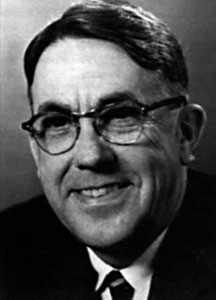
\includegraphics[width=\marginparwidth]{Source/images/arthur_samuel.jpg}
    \caption{Arthur L. Samuel (1901-1990) \cite{samuel-wikipedia} se graduó en Ingeniería Electrónica en el MIT. Trabajó en los laboratorios Bell, la Universidad de Illinois, en IBM y en la Universidad de Stanford (1966). Fue un pionero de los videojuegos y la inteligencia artificial. Popularizó el término <<Machine Learning>> en 1959. Implementó una IA para jugar a las damas, el primer caso  de éxito en aprendizaje automático. Contribuyó notablemente en el desarrollo de TeX.}
\end{marginfigure}

Fue en 1997 cuando Tom Mitchell propuso una definición más formal de aprendizaje \cite{tom-michell-machine-learning}, aproximada a la dada en el libro \textit{Learning from data} \cite{learning-from-data-1-2}, que exponemos en seguida.

El aprendizaje es un proceso por el cual se estima una dependencia desconocida (input-output) o la estructura de un sistema a partir de un número finito de observaciones.  El aprendizaje se compone de tres elementos principales: 

\begin{itemize}
    \item Un generador o función de distribución de la cual se extraen 
    vectores aleatorios 
    $x \in \mathbb R^ n$ 
    que dependen de una función de densidad desconocida \footnote{De hecho, encontrar esta función resolvería el problema de aprendizaje.}.
    
    \item Un sistema que produce un vector de salida $y$ por cada entrada del vector $x$ a partir del valor fijo $p(y|x)$, que es desconocido también. 
    
    \item Una \textit{learning machine}, que en el caso más general no es  más que un conjunto de funciones abstractas cuyos elementos son de la forma $f(x,w), w\in \omega$  (relaciones entre la entradas y el espacio de salidas posibles).
\end{itemize}

\begin{marginfigure}
    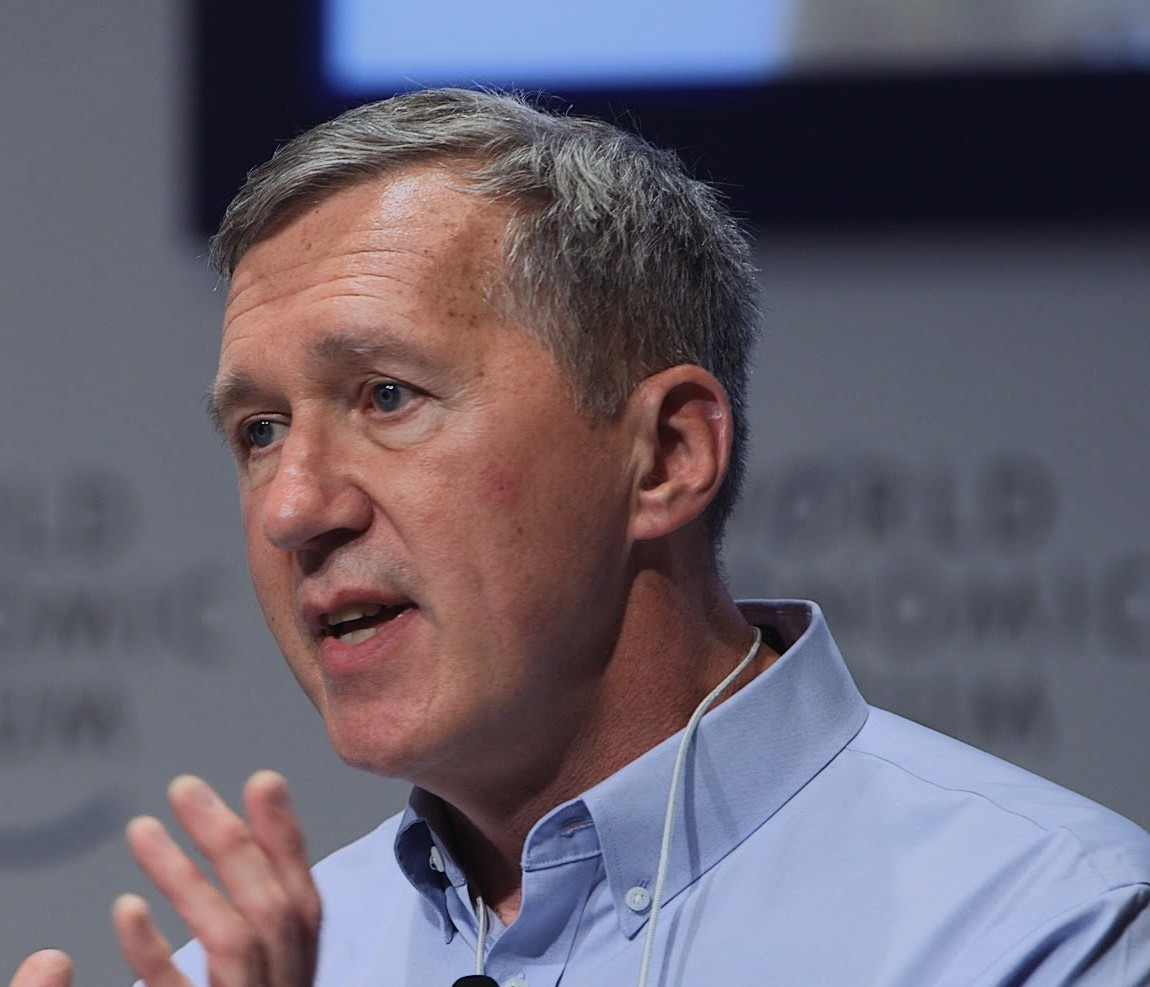
\includegraphics[width=\marginparwidth]{Source/images/tom_mitchell.jpg}
    \caption{Tom M. Mitchell (1951) estudió Ingeniería Electrónica en el MIT, se doctoró en la Universidad de Stanford y ejerce en la Univesidad de Carnegie Mellon. Es conocido por su libro de texto Machine Learning, una obra fundamental del campo del mismo nombre. Ha recibido numerosas condecoraciones y participa en asociaciones que promueven la ciencia y la ingeniería.}
\end{marginfigure}

Así pues, el objetivo del aprendizaje automático es encontrar una función que se aproxime a la función de densidad desconocida.

Por lo general la teoría se fundamenta en minimizar el error de estimadores, como el error cuadrático medio, ya que este se trata de un UMVUE  (estimador insesgado de mínima varianza). 

\begin{equation}
ECM = \frac{1}{n} \sum_{i=0} ^n (f(x_i) - y_i)^2,    
\end{equation}

donde $f(x_i)$ representa la predicción y $y_i$ la etiqueta de entrenamiento de $x_i$, es decir, su valor real. 

Objetivos similares se realizan también desde otros campos de la matemática como es el de teoría de la aproximación. 

No es habitual comenzar hablando del aprendizaje automático con teoría de la aproximación, pero en nuestro caso, que pretendemos centrarnos en redes neuronales. Esta teoría es fundamental para el Teorema de aproximación universal de las redes neuronales \cite{historia-aproximacion}.

\newpage
\section{Teoría de la aproximación. Teorema de aproximación de Stone-Weierstrass.}
El Teorema de Aproximación de Stone-Weierstrass es fundamental para el Aprendizaje Automático. Fue creado originalmente por Karl Weierstrass en 1885 y mejorado por Marshall Harvey Stone en 1937.

\begin{marginfigure}
    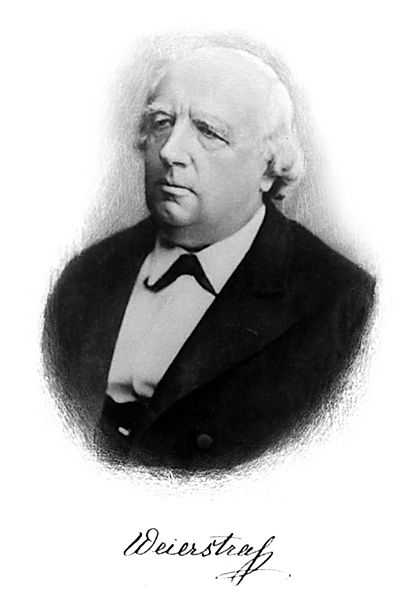
\includegraphics[width=\marginparwidth]{Source/images/weierstrass.jpg}
    \caption{Karl Weierstrass (1815-1897) \cite{weierstrass-wikipedia} fue un matemático alemán considerado el padre del análisis moderno. Entre sus logros más destacados figuran la definición de la continuidad de una función, demostrando el teorema del valor medio; y el teorema de Bolzano-Weierstrass usado posteriormente para estudiar las propiedades de funciones continuas en intervalos cerrados.}
\end{marginfigure}

\begin{marginfigure}
    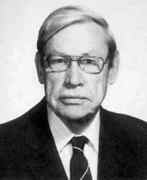
\includegraphics[width=\marginparwidth]{Source/images/marshall_stone.jpg}
    \caption{Marshall Harvey Stone (1903-1989) fue un matemático estadounidense que contribuyó al análisis, a la topología y al estudio de las álgebras booleanas. \cite{stone}.Generalizó  el enunciado del teorema de Weierstrass y simplificó su demostración en 1937.}
\end{marginfigure}

\begin{theorem}[Weierstrass, 1885]
    Para cualquier $\varepsilon > 0$ y para cualquier función $f$ continua sobre un intervalo $[a,b] \subset \mathbb{R}$ existe un polinomio con coeficientes reales, $p$, tal que 

    \begin{equation}
    \sup_{x \in [a,b]} |f(x) - p(x)| < \varepsilon        
    \end{equation}
\end{theorem}

\begin{theorem}[Stone-Weierstrass, 1937]
    Sea $K$ un subconjunto compacto de $\mathbb{R}^p$ y sea $\mathcal{A}$ una colección de 
    funciones continuas de $K$ a $\mathbb{R}$ con las siguientes propiedades: 

    \begin{enumerate}
        \item La función constantemente uno, definida como $e(x)=1$, para cualquier $x\in K$ pertenece a $\mathcal{A}$.
        \item Cerrado para sumas y producto para escalares reales. Si $f,g$ pertenece a  $\mathcal{A}$, entonces $\alpha f + \beta g$ pertenece a $\mathcal{A}$ . 
        \item Cerrado para producto. Para $f,g \in \mathcal A$, se tiene que $fg$ pertenece a $\mathcal{A}$. 
        \item Separación de $K$, es decir si $x \neq y$ pertenecientes a $K$, entonces existe una función $f$ en $\mathcal{A}$  de tal manera que $f(x) \neq f(y)$. 
    \end{enumerate}
    
     Se tiene que toda función continua de $K$ a $\mathbb{R}$ puede ser aproximada en $K$ por funciones de $\mathcal A$. 
\end{theorem}

% PERCEPTRÓN
\newpage
\section{El perceptrón}

\begin{marginfigure}
    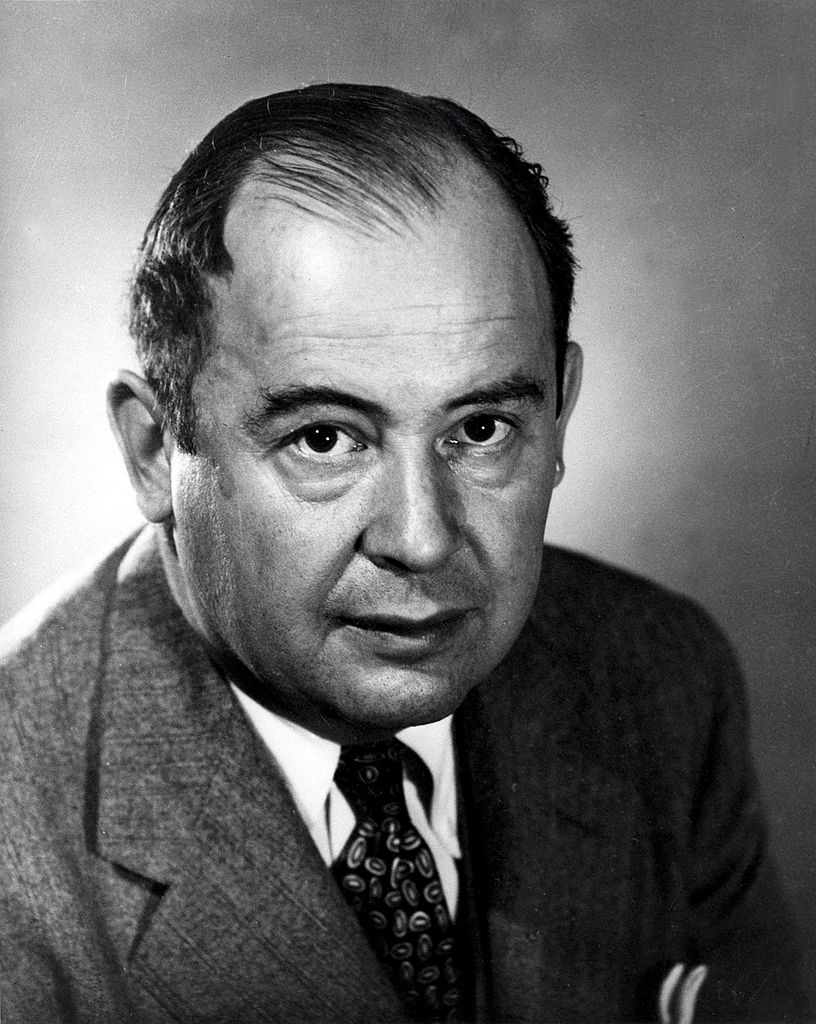
\includegraphics[width=\marginparwidth]{Source/images/Von_Neumann.jpg}
    \caption{John von Neumann (1903-1957) fue un matemático 
    húngaro-estadounidense conocido por el desarrollo de la arquitectura
    de computadores que lleva su nombre y que sigue utilizándose para el
    desarrollo de procesadores.}
\end{marginfigure}

En la historia de la Inteligencia Artifical, una de las preguntas que siempre ha existido
es la posibilidad de suplantar el pensamiento en una máquina utilizando leyes lógicas.
Esta pregunta tiene también otra interpretación: ¿Es posible modelar el pensamiento como 
un proceso mental gobernado por leyes lógicas? Esta pregunta es la que da lugar al
nacimiento de las redes neuronales y el aprendizaje profundo a partir del artículo
publicado en 1943 por Warren McCulloh y Walter Pitts. Titulado \textit{A Logical Calculus of the
Ideas Immanent in Nervous Activity}, formaliza la actividad nerviosa de las redes de 
neuronas en el cerebro humano mediante la lógica proposicional. Introduce el concepto de 
red neuronal artificial y algunas características como la actividad binaria de una neurona y la 
invariabilidad de la estructura de la red. Además, divide las neuronas en dos
grupos: las que en la actualidad se conocen como las neuronas de
entrada, y las neuronas de salida \cite{mcculloh-pitts}.

Este artículo serviría como inspiración no solamente para futuros trabajos en el campo de las redes neuronales, sino en la computación en general. John Von Neumann cita este artículo como una de sus inspiraciones más importantes en su trabajo \cite{skansi}. \\

\subsection{El perceptrón de Rosenblatt}
    En 1958, Frank Rosenblatt publica un artículo de vital importancia para el desarrollo del aprendizaje automático, titulado \textit{The Perceptron: A Probabilistic Model for Information Storage and Organization in the Brain}, \cite{rosenblatt}.
    
    \begin{marginfigure}
       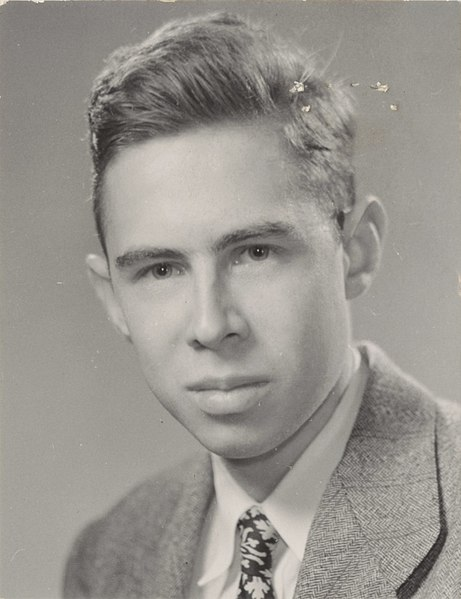
\includegraphics[width=\marginparwidth]{Source/images/rosenblatt.jpg}
        \caption{Frank Rosenblatt (1928-1971) fue un psicólogo estadounidense notable en el campo de la inteligencia artificial. Se graduó y doctoró en letras en la Universidad de Cornell. Trabajó en el Laboratorio Cornell Aeronáutico, donde fue sucesivamente psicólogo investigador, psicólogo senior y jefe de la sección de sistemas cognitivos. Allí fue donde llevó a cabo sus primeros trabajos sobre perceptrones, que culminaron en el desarrollo y construcción del harware del perceptrón Mark I, el primer ordenador que podría aprender habilidades nuevas a base de prueba y error.}
    \end{marginfigure}
    
    En este trabajo el autor intenta dar respuesta a dos preguntas básicas:
    \begin{enumerate}
        \item ¿Cómo se almacenada la información?
        \item ¿Cómo influye la información almacenada en la comprensión y en el comportamiento?
    \end{enumerate}
    
    En la época, había dos corrientes diferenciadas que intentaban responder a estas cuestiones:
    \begin{itemize}
        \item La corriente de la ``la memoria codificada'' sostenía que la información sensible se almacenaba de forma codificada. Debía existir alguna regla que a cada estímulo sensible le asociase un código que almacenar. El reconocimiento posterior de un nuevo estímulo suponía su codificación y comparación sistemática con otros códigos ya almacenados en busca de una respuesta.
        
        \item La corriente ``empiricista'' o ``conexionista'' defendía que no existía tal almacenamiento de códigos, sino que la información se almacenaba en forma de conexiones entre neuronas o canales de transmisión en el sistema nervioso. Un estímulo seguirá las conexiones apropiadas para él, activando la respuesta adecuada sin necesidad de otro proceso que lo reconozca o identifique.
    \end{itemize}
\restoregeometry
    En su artículo, Rosenblatt se alinea con el ``conexionismo''. Llama ``perceptrón'' a un hipotético sistema nervioso, que generaliza sistemas biológicos y máquinas.
    
    La \textit{Teoría del Perceptrón} se basa en las siguientes suposiciones desarrolladas por otros cientifícos de la época, entre los que destacan Hebb, Hayek, Uttley y Ashby.
    \begin{enumerate}
        \item Las conexiones físicas del sistema nervioso relacionadas
        con el aprendizaje y el reconocimiento no son idénticas entre 
        sujetos. La construcción inicial de una red neuronal es 
        mayormente aleatoria, sujeta a un mínimo de condiciones 
        genéticas.
        \item El sistema original de células conectadas tiene una
        cierta plasticidad. Tras un periodo de actividad neuronal,
        la probabilidad de que un estímulo en un conjunto de células
        provoque la respuesta de otro conjunto distinto es probable
        que cambie, debido a cambios en las neuronas.
        \item Por la exposición a grandes muestras de estímulos,
        estímulos ``similares'' tenderán a seguir caminos por las 
        mismas células, mientras que los ``distintos'' seguirán otros 
        caminos.
        \item La aplicación de refuerzos positivos y negativos puede
        facilitar o dificultar cualquier formación de conexiones
        en proceso.
        \item La similitud en estos sistemas se representa en algún 
        nivel del sistema nerviosos como la tendencia de que estímulos
        similares activen respuestas similares. Esta similitud no tiene
        por qué ser un atributo formal de cierta clase de estímulos,
        sino que depende de la organización específica de la red, que
        evoluciona conforme interacciona con el entorno. La estructura
        de la red afecta y determina las clases de ``cosas'' que 
        dividen el entorno que la red percibe.
    \end{enumerate}
    
    A partir de estas ideas, el autor expresa en términos matemáticos su teoría del funcionamiento de un perceptrón, que si bien no coincide exactamente con la definición formal que se usa en la actualidad, es una notable precursora.
    
    %Resumidamente, las conclusiones a las que llega Rosenblatt son las siguientes.
    %\begin{enumerate}
        %\item En un entorno con estímulos aleatorios, un sistema nervioso consistente en unidades %(neuronas) conectadas aleatoriamente puede aprender a asociar respuestas específicas a %estímulos específicos.
        
        %\item En un \textit{entorno ideal} \footnote{Rosenblatt llama \textit{entorno ideal} a aquel en %el que no hay tipos de estímulos diferenciados, todos tienen la misma naturaleza. Por ejemplo, %un entorno donde los únicos estímulos consisten en ver puntos de luz, en diferentes posiciones. %Por contra, en un \textit{entorno diferenciado} se pueden distinguir diferentes tipos o clases %de estímulos. Verbigracia, un entorno donde se pueden percibir cuadrados, círculos, triángulos %y letras del alfabeto.}, la probabilidad de una respuesta correcta disminuye acercándose al %funcionamiento aleatorio a medida que el número de estímulos aprendidos crece.
        
        %\item En un \textit{entorno ideal} no tiene sentido hablar de \textit{generalización} %\footnote{Entendemos por \textit{generalizacion} la capacidad del sistema nervioso de %identificar la clase a la que pertenece el estímulo}.
        
        %\item En un \textit{entorno diferenciado}, la probabilidad de que una asociación de estímulos %específicos aprendida sea correctamente retenida TODO
        
        %\item En un \textit{entorno diferenciado}, la probabilidad de que un estímulo que no ha sido %percibido con anterioridad sea reconocido y asociado a su clase apropiada (probabilidad de %generalización correcta) se aproxima a la misma asíntota
    %\end{enumerate}

\subsection{Noción actual de perceptrón}
    Los modelos actuales de redes neuronales, que explicamos más adelante, se componen de unidades mínimas, llamadas neuronas. La neurona más simple posible es el perceptrón, entendido como el modelo que presentamos a continuación.
    
    Un perceptrón \cite{yaser} es una función $h: \mathbb R ^ d \longrightarrow \{-1, 1\}$ definida por:
    \begin{equation}
     h(x) = sign( \sum_{i=1}^d w_i x_i + b ),
    \end{equation}
    donde $x = (x_1, \dots, x_d)$ son las entradas y $w_1, \dots, w_d$ son los pesos que se le asignan a las entradas.
    
    Intuitivamente, el perceptrón clasifica los posibles vectores de entrada $x$ en dos clases, $-1$ y $1$. Si consideramos los posibles vectores de entrada como puntos del plano, el perceptrón crea una recta que separa el plano en dos, dejando en una semiplano aquellos puntos que clasifica como $-1$ y en el otro semiplano los que clasifica como $1$. Pero esta separación no puede hacerse de cualquier manera, ya que en principio cada punto tendrá una clase verdadera y hay que conseguir que la clase que le asigne el perceptrón sea esa misma. Para ello necesitaremos ajustar los pesos $w_1, \dots, w_d$.
    
    \begin{figure}[!h]
        \centering
        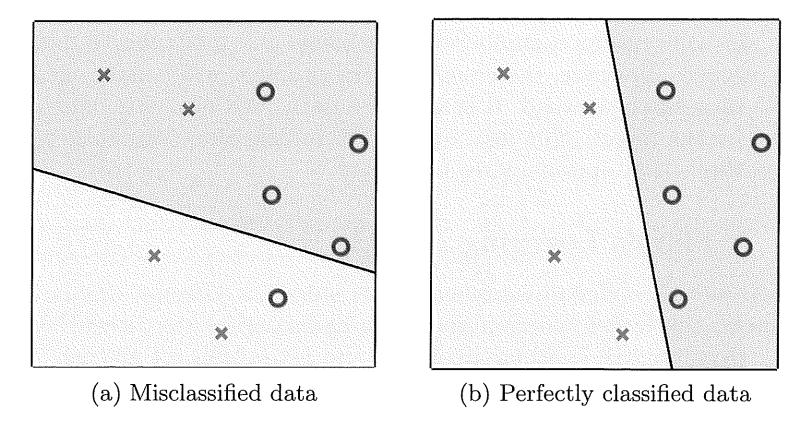
\includegraphics[height=20em]{Source/images/ajuste_pesos_perceptron.png}
        \caption{Ajuste de los pesos del perceptrón}
        \label{fig:ajuste_pesos_perceptron}
    \end{figure}
    
    En la figura \ref{fig:ajuste_pesos_perceptron} vemos dos posibles elecciones de pesos, la de la izquierda no consigue clasificar correctamente los puntos, mientras que la derecha sí.
    
    Por tanto, cabe preguntarse cuándo es posible encontrar los pesos adecuados y cómo hacerlo. La respuesta es sencilla: se puede hacer cuando las clases son linealmente separables y mediante el \textit{Algoritmo de Aprendizaje del Perceptrón}. Sin embargo a nivel práctico puede usarse el algoritmo, estableciendo algún criterio de parada, por ejemplo el número de iteraciones guardando el mejor peso o  cuando se encuentre uno cuyo error esté bajo un umbral. 
    
    El funcionamiento del susodicho algoritmo es el siguiente:
    \begin{enumerate}
        \item Partimos de unos valores iniciales ($t=0$) de los pesos, típicamente aleatorios cercanos a cero pero no nulos: $w(t) = (w_1(t), \dots, w_d(t))$.
        \item Si existe algún dato $x = (x_1, \dots, x_d)$ que no sea correctamente clasificado utilizando $w(t)$, actualizamos $w$: $w(t+1)=w(t) + h(x)y$.
        \item Repetimos el paso anterior mientras haya algún dato mal clasificado, cuando no lo haya finalizamos.
    \end{enumerate}
    Al finalizar la ejecución del algoritmo obtendremos los pesos buscados.
    
\newpage
\section{Perceptrón multicapa}

\subsection{Limitaciones del perceptrón. El problema XOR}  
El perceptrón de Rosenblatt tenía una limitación, que fue ilustrada
en 1969 en el libro de Marvin Minsky y Seymour Papert, \textit{
Perceptrons: An Introduction to Computational Geometry}. En él,
describían un fallo que habían cometido McCulloh y Pitts en su
trabajo de 1943: no habían tenido en cuenta la equivalencia como
función lógica, y expusieron lo que se conoce como el problema XOR.
\\

La función lógica XOR es la negación de la equivalencia, y se trata
de un problema no lineal. Minsky y Papert demostraron en su libro
que el perceptrón era incapaz de clasificar problemas no lineales.
Las consecuencias de este tratado fueron nefastas para el campo
de las redes neuronales, que se quedaron casi abandonadas hasta la
invención del perceptrón multicapa por David E. Rumelhart, Geoffrey
E. Hinton y Ronald J. Williams en 1986.

\subsection{El perceptrón multicapa de Rumelhart, Hinton y Williams}

Rumelhart, Hinton y Williams eran miembros y fundadores de un grupo de
investigación en la Universidad de San Diego en California, llamado
\textit{Parallel Distributed Processing (PDP)}. El objetivo inicial de este grupo
era realizar un compendio de todas las investigaciones relacionadas con
las redes neuronales que se habían realizado hasta la fecha. Sin embargo,
el grupo evolucionó, comenzando a realizar investigaciones que culminan con
la invención del perceptrón multicapa en 1986.
\\

El nombre de ``perceptrón multicapa'' es desafortunado, pues esta
invención no se trata de una concatenación de perceptrones, sino
de un nuevo sistema con un método de aprendizaje distinto. Este algoritmo fue denominado por los autores ``regla delta generalizada'' \cite{rumelhart-hinton-williams}, pieza clave en el posterior desarrollo
del algoritmo de retropropagación o ``backpropagation''.
\\

El perceptrón multicapa causó un auge de interés en las redes neuronales,
puesto que se trataba de una arquitectura capaz de solucionar problemas
no lineales, algo que todas las estructuras propuestas anteriormente
eran incapaces de resolver. La no linealidad en la estructura brinda la posibilidad
también de obtener representaciones internas complejas de entidades, una
característica muy importante a la hora de representar fenómenos complejos que
son comunes en el pensamiento humano, como el lenguaje. Sin embargo,
ninguno de los autores presentó evidencias de que el cerebro aprende mediante la
regla delta generalizada. Aunque pudiera parecer un problema menor, se trata de un 
asunto de importancia crítica a la hora de realizar modelos de cognición que
intenten ser plausibles biológicamente, que era el objetivo del PDP \cite{multilayer}. El modelo de aprendizaje cerebral humano sigue siendo en la actualidad un tema de debate, puesto que todavía no se ha llegado a un consenso.

\subsection{Definición del perceptrón multicapa}

El perceptrón multicapa clásico se define como el conjunto de los siguientes
elementos:\\

\begin{figure}[!h]
    \centering
    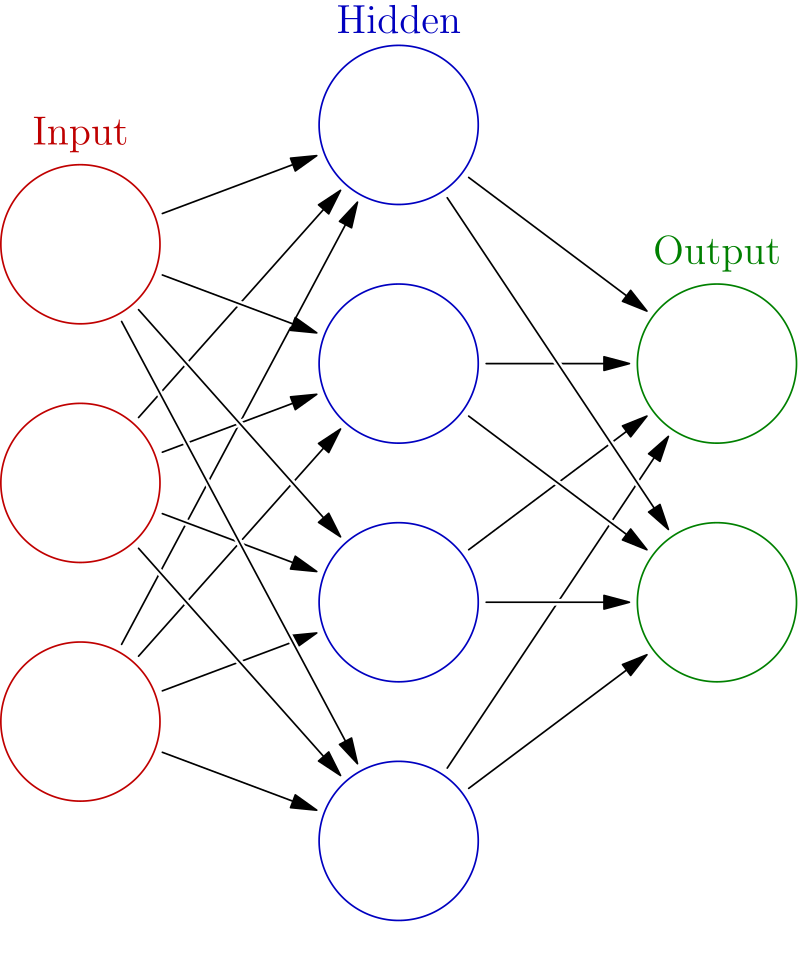
\includegraphics[height=20em]{Source/images/multicapa.png}
    \caption{Perceptrón multicapa con una capa oculta}
    \label{fig:multicapa}
\end{figure}

\begin{itemize}
    \item Una función lineal que agrega las entradas y produce una salida.
    \begin{equation}\label{agregacion}
        z=f(x_n,w_n)=b+\sum_i^nx_iw_i
    \end{equation}
    donde
    \begin{itemize}
        \item $z$ es la salida.
        \item $b$ es una constante.
        \item $x_i$ son las entradas a la neurona.
        \item $w_i$ son los pesos de cada una de las entradas.
    \end{itemize}
    \item Una función de activación sigmoidal.
    \begin{equation}
        a=\sigma(z)=\frac{1}{1+e^{-z}}
    \end{equation}
    El objetivo de esta función es eliminar la linealidad de la salida.
    \item Una función umbral en los problemas de clasificación.
    \begin{equation}
        \hat{y}=f(a)=
    \begin{cases}
        1 & \text{si}\quad a>0.5 \\
        -1 & \text{en cualquier otro caso}
    \end{cases}
    \end{equation}
    O una función identidad en los casos de regresión 
    \begin{equation}
        \hat{y}=f(a)=a
    \end{equation}
    \item Una función de costo que computa el error total producido por la red. Esta
    función se trata de la suma de los errores cuadráticos:
    \begin{equation}\label{f_costo}
        E=\frac 12 \sum_k(\hat{y}_k-y_k)^2
    \end{equation}
    donde
    \begin{itemize}
        \item $\hat{y}_k$ es la predicción del $k$-ésimo ejemplo.
        \item $y_k$ es el resultado real del $k$-ésimo ejemplo.
    \end{itemize}
    \item Un método de aprendizaje para realizar cambios en los pesos: regla
    delta generalizada.
\end{itemize}

\subsection{La regla delta generalizada}

Aunque se atribuya la regla delta generalizada a Rumelhart, Hinton y Williams,
fue descubierta por primera vez por Paul Werbos en su tesis doctoral. No
obstante, este descubrimiento pasó desapercibido. Fue descubierta por segunda
vez por David Parker en 1981, que intentó obtener una patente para el
descubrimiento. Acabó publicando su descubrimiento en 1985. La tercera y
última vez que fue descubierta fue de forma independiente por Yann LeCun en
1985 y Rumelhart, Hinton y Williams en 1986 \cite{skansi}.\\

El proceso de esta regla es el siguiente:

\begin{enumerate}
    \item Se realiza una prueba, es decir, se envía una entrada al perceptrón
    y se recoge la salida final.
    \item Se compara el error realizado por la capa de salida usando la 
    función costo definida anteriormente en (\ref{f_costo}).
    \item Ese error es utilizado para modificar los pesos de sus conexiones
    con la capa anterior. La modificación es la siguiente:
    \begin{equation}
        \Delta w_i=\eta(\hat{y}-y)\sigma'(z)x_i
    \end{equation}
    Estos tres primeros pasos son idénticos a realizar un descenso de 
    gradiente en un perceptrón.
    \item Para cada capa oculta, en orden descendente, se computa el error,
    que no es más que la suma de todos los errores de las neuronas de la
    siguiente capa que están conectadas con ella. Esto es, si una red
    tiene tres capas ocultas, el error de la tercera neurona de la segunda
    capa es la suma de los errores de las neuronas de la tercera capa que
    tienen como entrada la salida de la neurona en cuestión. Cada uno de
    los pesos de esa neurona se modifica de la misma manera que los de
    la capa de salida \cite{deltarule-process}.
\end{enumerate}
 
 Una de las propiedades más interesantes e importantes de esta regla es que
 es capaz de detectar correlaciones entre vectores linealmente independientes,
 mientras que las reglas anteriores eran incapaces de detectar este tipo
 de patrones \cite{deltarule-advantages}. 

\newpage
\section{Redes neuronales hacia delante. Retropropagación.}

Las redes neuronales hacia delante o ``feed-foward neural networks'' (FFNNs) son
las redes neuronales más usadas y las primeras en ser utilizadas. En ellas, las
entradas siguen una única dirección (hacia delante), desde la capa de entrada
hasta la capa de salida, pasando, si hay, por las capas ocultas. Es en este tipo de
redes en las cuales se incluye el perceptrón y el perceptrón multicapa descritos 
anteriormente.\\

\begin{figure}[!h]
    \centering
    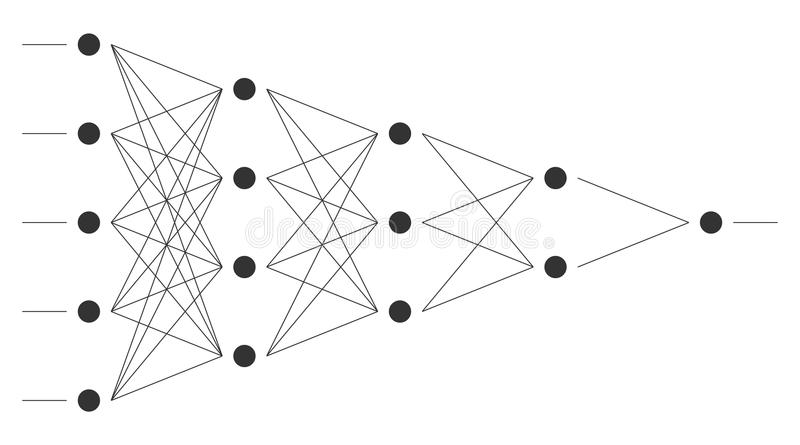
\includegraphics[width=0.7\textwidth]{Source/images/feedfowardnet.jpg}
    \caption{Ejemplo de estructura de una FFNN con cinco entradas y una salida}
    \label{fig:feedfowardnet}
\end{figure}

Cabe resaltar que el concepto de una red neuronal
no cíclica es muy anterior al de perceptrón multicapa, pudiéndose remontar al primer
artículo sobre neuronas artificiales de 1943 del que se ha hablado ya anteriormente,
en el que en la segunda sección se describe la teoría lógica de redes neuronales 
``sin círculos'' \cite{mcculloh-pitts}. En el campo del Aprendizaje Profundo, la 
primera publicación de una red neuronal hacia delante es la publicada en 1968 por 
Alexey Ivakhnenko y el GMDH (\textit{Group Method of Data Handling}), usando una 
estructura de perceptrones de varias capas \cite{jurgen}.\\

En la actualidad, las redes neuronales hacia delante que se utilizan están basadas
en el perceptrón multicapa, aunque con ciertas generalizaciones. La función de
activación puede ser otra función aparte de la sigmoide. Se suelen usar las
siguientes funciones de activación:\\

\paragraph{Sigmoide}
\begin{equation}
    \sigma(x)=\displaystyle\frac{1}{1+e^{-x}}
\end{equation}

\begin{figure}[!h]
    \centering
    \begin{tikzpicture}[scale=0.6]
        \begin{axis}[
            axis on top = true,
            axis x line = bottom,
            axis y line = left,
            grid = major,
            xlabel = $x$,
            ylabel = $\sigma(x)$,
        ]
            \addplot[
                red,
                domain = -5:5,
                samples = 100
            ]
                {1/(1+exp(-x))};
        \end{axis}
    \end{tikzpicture}
    \caption{Gráfica de la sigmoide}
\end{figure}

La función sigmoide o logística es la función de activación clásica. Se trata
de una función diferenciable, lo que la hace cómoda a la hora de utilizar
retropropagación. Se suele utilizar en modelos donde la salida es una
probabilidad, puesto que la imagen está acotada entre cero y uno. Sin embargo,
esta función sufre del problema de desvanecimiento de gradiente . 
Además, la salida de todas las neuronas tiene el mismo signo (positivo), lo que
puede dificultar el aprendizaje y hacerlo más inestable \cite{activation}.\\

\paragraph{Softmax}
\begin{equation}
f(x)_i=\displaystyle\frac{e^{x_i}}{\sum_j^n e^{x_j}},\quad
x=(x_1,\ldots,x_n)
\end{equation}

Cuando tenemos un problema de clasificación multidimensional, para unos valores
de entrada, queremos saber a que clase es más probable que pertenezcan esos
valores. Es en esos casos en los que usamos esta función de activación. Se
trata de una generalización de la sigmoide a varias dimensiones, por lo que
la imagen de cada componente $x_i$ se puede interpretar como una probabilidad
relativa. Es por ello que se suele utilizar en las neuronas de la capa de
salida.\\

\paragraph{Tangente hiperbólica}
\begin{equation}
    \tanh(x)=\displaystyle\frac{e^x-e^{-x}}{e^x+e^{-x}}
\end{equation}

\begin{figure}[!h]
    \centering
    \begin{tikzpicture}[scale=0.6]
        \begin{axis}[
            axis on top = true,
            axis x line = bottom,
            axis y line = left,
            grid = major,
            xlabel = $x$,
            ylabel = $\tanh(x)$,
        ]
            \addplot[
                red,
                domain = -5:5,
                samples = 100
            ]
                {(exp(x)-exp(-x))/((exp(x)+exp(-x))};
        \end{axis}
    \end{tikzpicture}
    \caption{Gráfica de la tangente hiperbólica}
\end{figure}

Esta función es muy similar a la sigmoide, con la diferencia de que está
centrada alrededor del origen y su imagen está acotada entre $[-1,1]$.
Esto hace que se puedan clasificar sus salidas como ``muy positivas'',
``neutrales'' y ``muy negativas''. Se suele utilizar en las neuronas de las
capas ocultas puesto que la media de las imágenes es cercana a cero, ayudando a
centrar los datos. Como la sigmoide, la tangente hiperbólica sufre del problema
de desvanecimiento de gradiente \cite{activation}.\\

\paragraph{ReLU}
\begin{equation}
    ReLU(x)=\max(0,x)
\end{equation}

\begin{figure}[!h]
    \centering
    \begin{tikzpicture}[scale=0.6]
        \begin{axis}[
            axis on top = true,
            axis x line = bottom,
            axis y line = left,
            grid = major,
            xlabel = $x$,
            ylabel = $ReLU(x)$,
        ]
            \addplot[
                red,
                domain = -5:0,
                samples = 100
            ]
                {0};
            \addplot[
                red,
                domain = 0:5,
                samples = 100
            ]
                {x};
        \end{axis}
    \end{tikzpicture}
    \caption{Gráfica de la ReLU}
\end{figure}

ReLU, también llamado Rectificador Lineal, es una función muy eficiente
computacionalmente, puesto que únicamente activa las neuronas si 
(\ref{agregacion}) es positiva. Además, acelera la convergencia del gradiente
debido a su propiedad lineal. Sin embargo, la ventaja de esta función es
además su desventaja: para valores negativos, el gradiente es cero, por lo
que en el algoritmo de retropropagación algunas neuronas no actualizan sus
pesos, convirtiéndolas en ``neuronas muertas'' \cite{activation}. El 
Rectificador Lineal como función de activación, aunque de expresión muy 
distinta, tiene un fundamento biológico y matemático \cite{relu}.\\

\paragraph{ELU}
\begin{equation}
    ELU(x)=\begin{cases}
        x & \quad x>0 \\
        \alpha(e^x-1) & \quad x\leq 0 
    \end{cases},\quad\alpha>0
\end{equation}

\begin{figure}[!h]
    \centering
    \begin{tikzpicture}[scale=0.6]
        \begin{axis}[
            axis on top = true,
            axis x line = bottom,
            axis y line = left,
            grid = major,
            xlabel = $x$,
            ylabel = $ELU(x)$,
        ]
            \addplot[
                red,
                domain = -5:0,
                samples = 100
            ]
                {1.2*(exp(x)-1)};
            \addplot[
                red,
                domain = 0:5,
                samples = 100
            ]
                {x};
        \end{axis}
    \end{tikzpicture}
    \caption{Gráfica de la ELU ($\alpha=$1.2)}
\end{figure}

La función ELU, ``Exponential Linear Unit'' es una modificación del
Rectificador Lineal que elimina el problema de las neuronas muertas. Sin
embargo, aumenta el coste de computación al contener una exponencial y contiene
un parámetro $\alpha$ fijo, que no ``aprende'' \cite{activation}.\\

El problema de desvanecimiento de gradiente, mencionado en la
función sigmoide y la tangente hiperbólica, es el siguiente: Puesto 
que el algoritmo de retropropagación usa la regla de la cadena, para
funciones cuyo gradiente está en un intervalo cercano al cero, el 
valor del gradiente se va reduciendo exponencialmente conforme se va
propagando, por lo que los pesos de las primeras capas se apenas se 
modifican, llegando incluso a permanecer intactos \cite{vanishing}.

\subsection{Retropropagación o ``backpropagation''}

El algoritmo de aprendizaje que se usa en la actualidad en las redes 
neuronales hacia delante está basado en la regla delta generalizada descrita 
en 1986 por Rumelhart, Hilton y Williams. Sin embargo, el concepto es muy
anterior. Nace en los años 1960 dentro del campo de la teoría de control de
la mano de Henry K. Kelley \cite{kelley}. La versión actual fue propuesta
por Yann LeCun en su tesis doctoral de 1987, \textit{	
Modèles connexionnistes de l'apprentissage}. El objetivo de este algoritmo es 
calcular el gradiente de los pesos en cada una de las capas de la red, en 
orden descendente, y actualizar los pesos de manera que el error se minimice.
Es decir, se trata de realizar, para cada peso $w$:
\begin{equation}
    w_{\text{nuevo}}=w_{\text{antiguo}}-\eta\bigtriangledown E
\end{equation}    
donde $\eta$ es la tasa de aprendizaje y $E$ la función de costo.

\subsection{Teorema de aproximación universal}

Todos los modelos presentados pueden suscitar dudas sobre si
realmente son capaces de aproximarse o incluso converger a la
solución del problema que se plantea. Esto es, si un modelo es capaz
de encontrar la regla o patrón subyacente en los datos con los que
trabaja. En 1989, Kurt Hornik de la Universidad de Viena, y Maxwell 
Stinchcombe y Halbert White de la Universidad de San Diego en 
California demostraron que sí lo hacen. \\

El artículo ``establece que las redes neuronales hacia delante 
comunes con tan sólo una única capa oculta usando una función de 
activación sigmoidal arbitraria son capaces de aproximar cualquier 
función boreliana medible que vaya de un espacio de dimensión finita
a otro con el grado de precisión que se desee, siempre que haya 
suficientes capas ocultas. En este sentido, las redes neuronales 
hacia delante son aproximadores universales.'' 
\cite{aproximator-original}. \\

Otra manera más intuitiva de enunciar lo que el artículo demuestra 
es la siguiente: Para cualquier función continua $f$ en un
conjunto $K$ compacto, existe una red neuronal hacia delante con una
única capa oculta que aproxima $f$ con un error arbitrario 
$\epsilon>0$ en $K$ \cite{aproximator}.\\

En 1991, Kurt Hornik demuestra que no es incluso necesario que la
función de activación sea sigmoidal, sino que únicamente es
necesario que la función sea acotada y no constante para que la
red neuronal sea aproximadora universal. Además, da condiciones que
aseguran que una red neuronal hacia delante es capaz de aproximar
funciones y sus derivadas si poseen funciones de activación 
suficientemente suaves \cite{aproximator-nonsigmoid}. \\

Una generalización más ocurre en 1993, cuando Moshe Leshno y otros
demuestran que las redes neuronales hacia delante son aproximadoras
universales si y sólo si tienen funciones de activación no 
polinómicas \cite{aproximator-nonpolinom}.

\newpage
\section{ Redes neuronales profundas.}
La redes neuronales profundas no son  más que una red de neuronas con varias capas ocultas. En la actualidad no se ha dado una definición formal al respecto ni tampoco se tiene claro a partir de cuántas capas ya debiera considerarse <<profunda>>. \\

Cabe hacerse la siguiente pregunta: Si con una capa, gracias al teorema de aproximación universal de las redes neuronales sabemos que es convergente, ¿por qué deberíamos utilizar más? \\ 

El uso de una capa fue el estándar hasta aproximadamente el año 2005, cuando de manera empírica se observaban resultados más favorables en redes con más capas  \cite{numero-capas} (de hecho este artículo que estudia sobre el la mejora que se produce introduciendo capas ocultas fue publicado en 2020). El motivo de esto es aún desconocido y es que como apuntan investigadores como Pablo Mesejo: los grandes teoremas sobre las redes neuronales aún están por descubrir. 

\subsection{Otros retos aún por resolver}

Debido a los recientes y rápidos avances de las redes neuronales
en los últimos tiempos, su uso en tanto productos comerciales e
investigación está en expansión constante. Un ejemplo podría ser
el uso de aprendizaje profundo para el desarrollo de sistemas de 
automoción autónomos. Es en estos casos donde uno de los mayores
problemas sin resolver, la incertidumbre acerca de un resultado
a partir de datos nuevos, es de crítica importancia. \\

Las redes neuronales obtienen sus resultados de manera inductiva,
mientras que los algoritmos tradicionales siguen un método deductivo
a partir de reglas y patrones. No se puede explicar qué hace una red
neuronal en cada una de sus capas de manera general. Existen maneras
de ``explicar'' los resultados de clasificadores, como LIME \cite{lime}, pero explican el resultado específico, no la regla
general.\\

Otro de los retos tiene que ver con los modelos en los que se usan
las redes neuronales, que suelen carecer de especificaciones acerca
de los requisitos y el diseño, además de una falta de robustez
\cite{security-neuralnets}.
Esta falta de robustez es de vital problemática en los 
clasificadores de imágenes, en los que un pequeño cambio en las
entradas, muchas veces imperceptible al ojo humano, provoca cambios
radicales en el resultado \cite{image-class}.

\newpage
\margenimagen
\section {Tipos de redes neuronales profundas}
    \begin{minipage}{0.9\linewidth}
        \vspace{5pt}%margen superior de minipage
             \begin{flushright}
            
        {\small
            \textit{All models are wrong, but some are useful.}
        }
        \vspace{5pt}%margen inferior de la minipage
         George Box.
        \end{flushright}
    \end{minipage}

Ante un problema de aprendizaje automático, se debe tener en cuenta la naturaleza del mismo.:
\begin{itemize}
    \item Tipo de aprendizaje: supervisado, no supervisado, clustering...
    \item Objetivo: clasificación, búsqueda de patrones...
\end{itemize} 

Como resultado de la diversidad de problemas que se pretenden resolver 
surge una gran variedad de redes neuronales profundas \cite{tipos-general-redes-neuronales-profundas}, aquí expondremos las más importantes. 

\begin{marginfigure}
    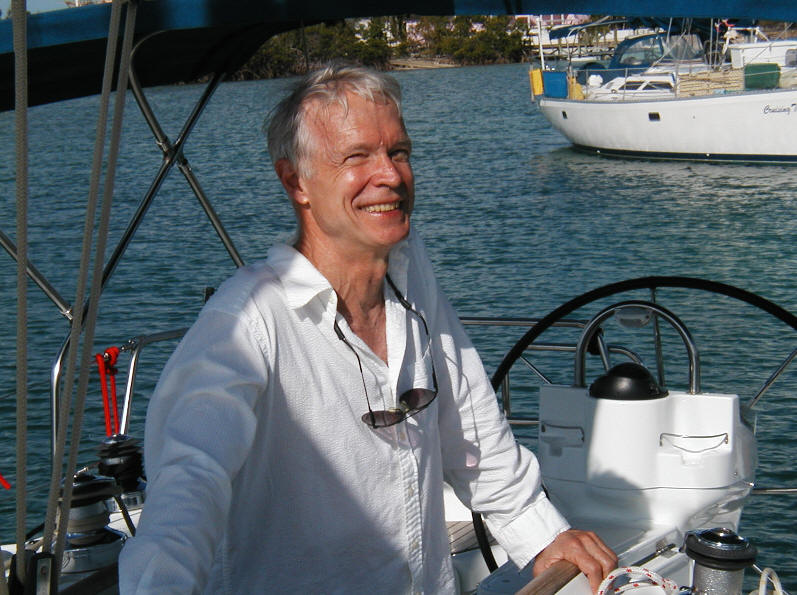
\includegraphics[width=\marginparwidth]{Source/images/John_Hopfield.jpg}
    \caption{John Hopfield (1933) \cite{hopfield} es un físico polaco. Trabajó en los laboratorios Bell, la universidad de Pricenton, la universidad de Berkeley y el Instituto Tecnológico de California en temas relacionados con la física, biología molecular y neurociencia.}
    \label{fig:RegistrationComponents}
\end{marginfigure}

\subsection{Red recurrente, red de tensor neural o RNTN}

%%%% De la wikipedia   
Las redes recurrentes  \ref{fig:Esquema del RNN} fueron propuestas por primera vez por John Hopfield en 1982 y desarrolladas gracias a las aportaciones de David Rumelhart en 1986.

Una idea intuitiva y bioinspirada sería pensar en el proceso de pensamiento humano, que realiza síntesis a partir de experiencias, pensamientos o información anterior. No toda pensamiento surge de la nada. 

\begin{marginfigure}
    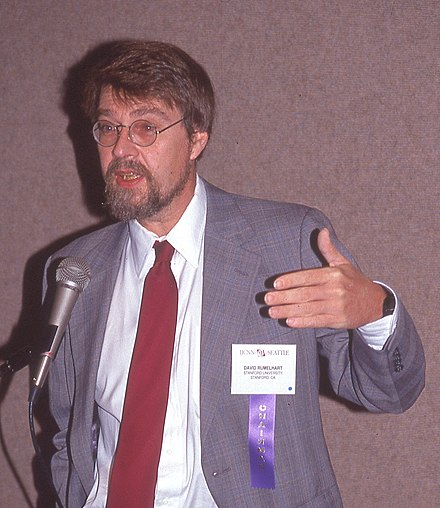
\includegraphics[width=\marginparwidth]{Source/images/David_Rumelhart.jpg}
    \caption{David Rumelhart (1942 - 2011) \cite{Rumelhart} fue un psicólogo estadounidense que trabajó en el campo de la modelización matemática de la psicología, la inteligencia artificial simbólica y el conexionismo.}
\end{marginfigure}

Estas redes utilizan grafos dirigidos o no dirigidos basados en secuencias temporales. Se utilizan para el reconocimiento de voz, el procesamiento de texto, el análisis de sentimientos, el análisis y el reconocimiento de la entidad de nombre. 

Existen multitud de infraestructuras, como las CTRNN,  basadas en sistemas de ecuaciones diferenciales ordinarias y que utilizaremos de ejemplo.

  \begin{figure}[htb]
        \centering
        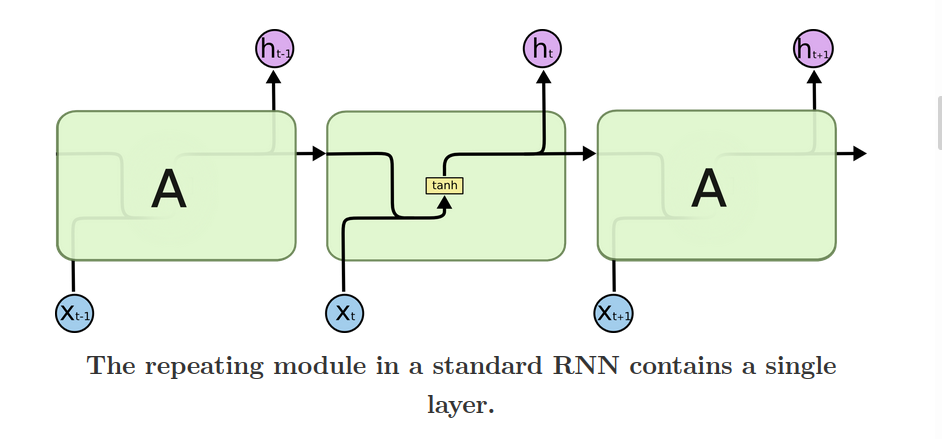
\includegraphics[width=0.75\textwidth]{Source/images/RNN.png}
        \caption{Esquemas de las RNN, \ref{fig:diagrama}}
        \label{fig:Esquema del RNN}
    \end{figure}
\newpage\restoregeometry

Para cada neurona $i$-ésima que recibe como activación $y_i$ su tasa de cambio viene dada por: 

\begin{equation}
\tau _i \dot{y}_i = -y_i + \sum_{j=1}^n w_{i,j} \sigma( y_j - \Omega _ j) + I_ i(t),   
\end{equation}

donde:
\begin{itemize}
\item $\tau_i$ es una constante del tiempo postsináptico. 
\item $y_i$ nodo activación postsináptica.
\item $\dot{y}_i$ Ratio de activación del nodo psináptico. 
\item $w_{j,i}$ peso de las conexiones. 
\item $\sigma$ sigmoide.
\item $y_i$ nodo activación presináptica.
\item $\Omega_j$ sesgo de la conexión presináptica. 
\item $I_i(t)$ input del nodo (si es que hay). 
\end{itemize}

Destacan además las redes LTSM que tratan de resolver uno de los problemas fundamentales de las redes recurrentes: que los pesos anteriores pesen demasiado en el modelo impidiendo actualizaciones útiles nuevas. 

\subsubsection{Redes LSTM}  

\cite{LSMTM-web} 

Las redes \textit{Long Short Term Memory} \cite{LSMTM-paper} capaces de aprender de experiencias a largo plazo. 

Son de gran utilidad en procesado de texto, un ejemplo sería, si quisiéramos  predecir la palabra a continuación de  \textit{ Las nubes están en el }, necesitaremos información de las palabras anteriores a la que queremos predecir.  


  \begin{figure}[!h]
        \centering
        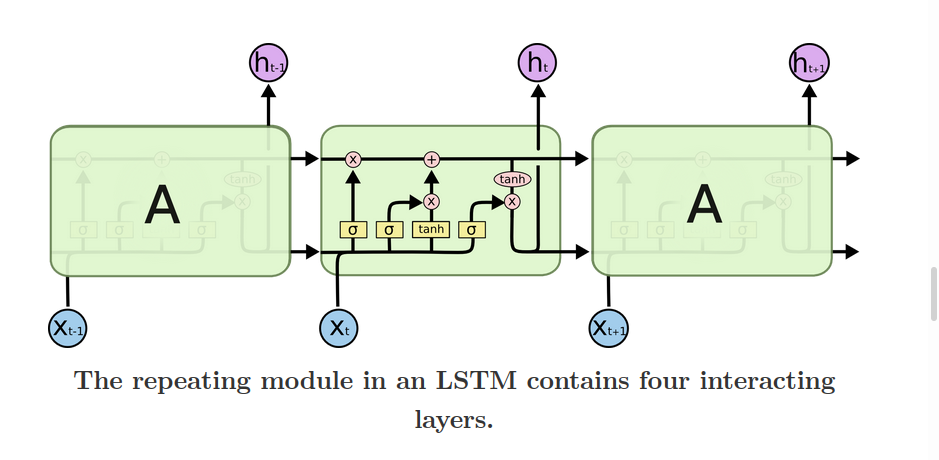
\includegraphics[width=\textwidth]{Source/images/LSTM.png}
        \caption{Esquemas de las LSTM \ref{fig:diagrama}}
        \label{fig:Esquema del LSTM}
    \end{figure}
    
    \begin{figure}[!h]
        \centering
        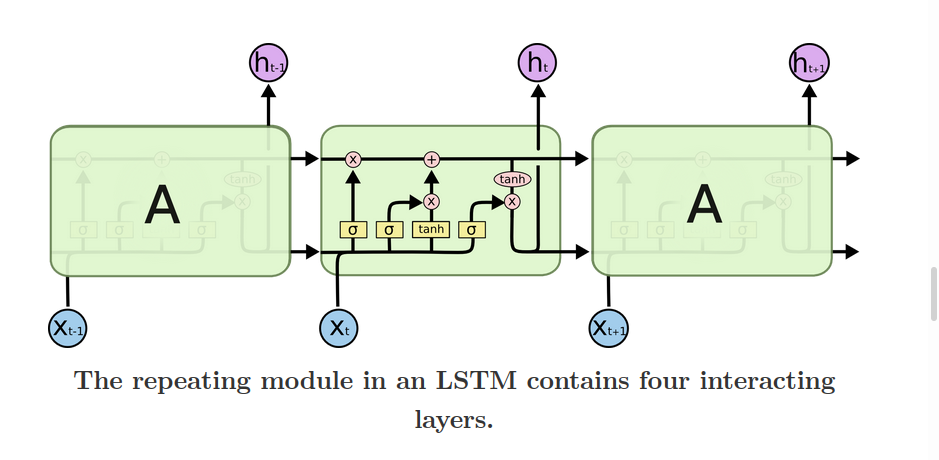
\includegraphics[width=\textwidth]{Source/images/LSTM.png}
        \caption{Esquemas de las LSTM}
        \label{fig:diagrama}
    \end{figure}

Puede verse un esquema de su diseño en la figura \ref{fig:Esquema del LSTM}. 

La idea central del diseño es la siguiente: 

La existencia de una célula de estado $C_t$ ( en la iteración $t$), para calcular $C_t$ a partir de $C_{t-1}$ y la etiqueta son necesarios los siguientes cálculo auxiliares 

\begin{equation}
    f_t = \sigma (W_f [h_{t_1}, x_t] + b_f)
\end{equation}

\begin{equation}
i_ t = \sigma (W_i [h_{t_1}, x_t] + b_i)
\end{equation}

\begin{equation}
 \Tilde{C}_t = tanh(W_c [h_{t_1}, x_t] + b_c)
\end{equation}

Hasta que finalmente obtenemos

\begin{equation}
 \Tilde{C}_t = f_t * C_{t-1} + i_t * \Tilde{C}_t
\end{equation}

Para la salida del modelo $h_t$ se calcula como   

\begin{equation}
 \Tilde{h}_t = o_t * tanh(C_t)
\end{equation}
Donde 
\begin{equation}
 \Tilde{h}_t = \sigma ((W_o[h_{t_1}, x_t] + b_0)) 
\end{equation}   

\subsubsection{GRU}  

Otra variable creada con la misma idea que LSTM son las GRU, \textit{Gated recurrent unit} que fueron introducidas en 2014 por Kyunghyun Cho. 

Un esquema de GRU es \ref{fig:esquema-GRU} \cite{GRU-web} que se diferencia de las LSTM por tener menor número de parámetros y carecer de \textit{gated output}. 
\margenimagen
    \begin{figure}[!h]
        \centering
        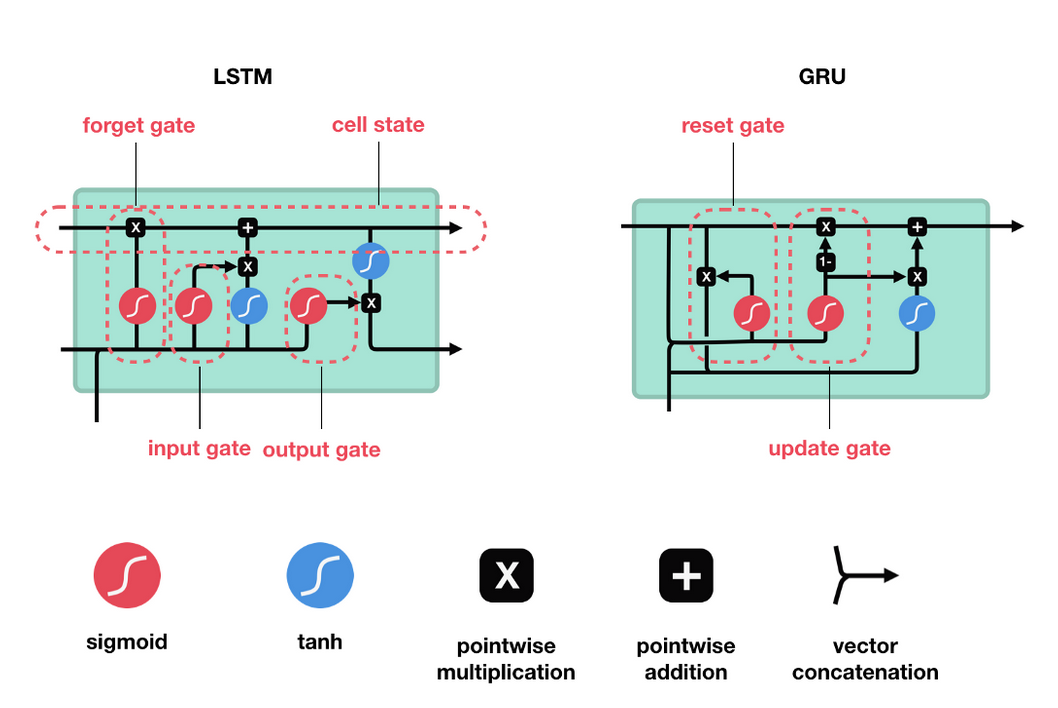
\includegraphics[width=0.8\textwidth]{Source/images/GRU.png}
        \caption{Esquema GRU}
        \label{fig:esquema-GRU}
    \end{figure}
\begin{marginfigure}
    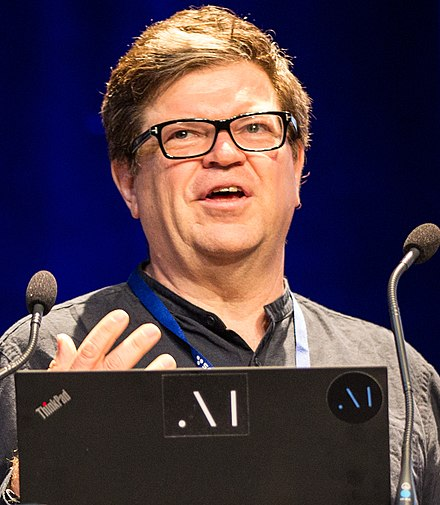
\includegraphics[width=\marginparwidth]{Source/images/Yann_LeCun.jpg}
    \caption{Yan LeCun nació en Francia en 1961. Ha trabajado en el aprendizaje automático, la visión por computador, los robot móviles y la neurociencia computacional. En 2018 ganó el premio Turing y es considerado junto con Geoffrey Hinton y Yoshua Begio el padrino del aprendizaje profundo. Actualmente trabaja como investigador en inteligencia artificial en Meta Platforms (antiguo Facebook).}
\end{marginfigure}

Se utilizan para ciertas tareas como modelos de música polifónicos, reconocimiento de voz y procesamiento de lenguaje natural.  
\cite{GRU-wikipedia}.  

(La formalización matemática se puede hacer siguiente el mismo esquema que la anterior o consultando directamente \cite{GRU-wikipedia}). 

\subsection{Red convolucional o CNN}

Las redes neuronales convolucionales (CNN), también conocidas como ConvNets, son redes neuronales profundas para el procesamiento y detección de objetos. Fueron desarrolladas pro Yann LeCun en 1988, que él llamó LeNet y las utilizó para el reconocimiento de características como el código ZIP y dígitos.

\subsection{Red generativa antagónica o GAN}
Este tipo de redes se usan para la generación de contenido multimedia. Por ejemplo, la reconstrucción de imágenes y \href{https://thispersondoesnotexist.com}{la generación de rostros que parezcan reales} \cite{gan-explanacion}. Fueron creadas por Ian Goodfellow y sus compañeros en junio de 2014.

\begin{marginfigure}
    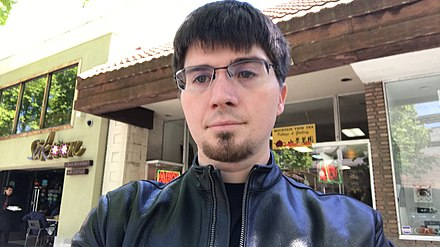
\includegraphics[width=\marginparwidth]{Source/images/Ian_Goodfellow.jpg}
    \caption{Ian Goodfellow (1986) es un ingeniero informático estadounidense. Trabajó en Google como parte del equipo de Google Brain, después pasó a formar parte de OpenAI y actualmente trabaja para Apple.}
\end{marginfigure}

Su diseño es el siguiente: 
Se tienen dos redes neuronales profundas que son <<adversarias>> en un juego de suma cero. Una de ellas realiza la tarea de \textit{Discriminador} y la otra la tarea de \textit{generador} .

\newpage\restoregeometry

\begin{figure}[!h]
\center
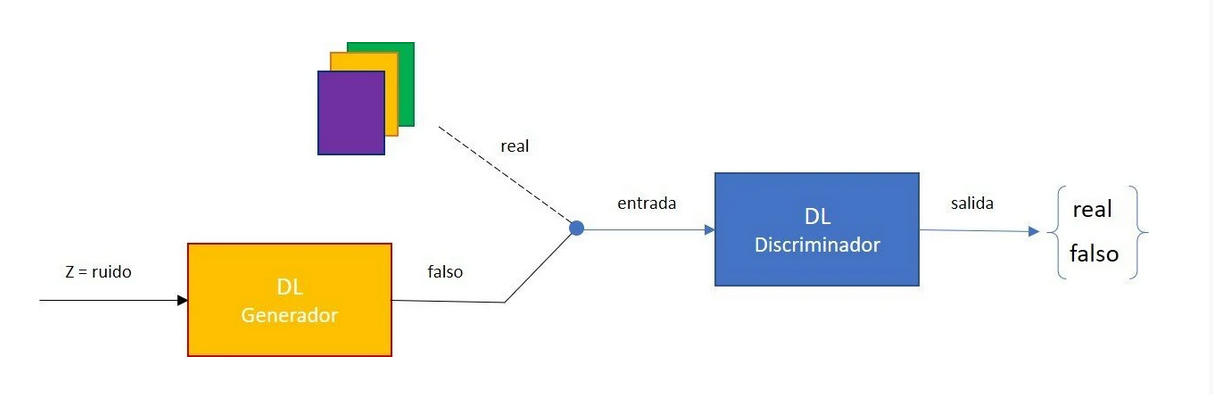
\includegraphics[width=\textwidth]{Source/images/GAN.png}
\caption[GAN]{Imagen explicativa del GAN}
\end{figure}

Para entrenar esta arquitectura se necesita un conjunto de datos 
reales, de esta forma cuando le pasemos una foto real al 
discriminador esta deberá de ser tomada como correcta. El generador 
deberá actualizar sus pesos hasta que el discriminador tome sus 
fotos generadas como buenas.

\newpage\margenimagen

\section{Optimización de Redes Neuronales}
    A la hora de calcular los pesos del perceptrón, podemos seguir el método de regresión lineal esto es, minimizar el error cuadrático medio mediante derivación. Sin embargo, este método tiene la debilidad de no ser eficiente para dimensiones elevadas, especialmente en casos en los que la función de coste (error cuadrático medio) tiene más de un mínimo local. De aquí surge la necesidad de buscar otros métodos, como el método del descenso de gradiente.

    \subsection{Método de regresión lineal}
    
        \begin{marginfigure}
        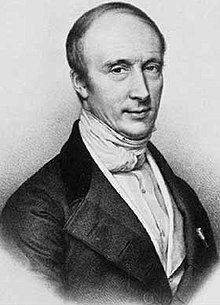
\includegraphics[width=0.5\marginparwidth]{Source/images/cauchy.jpg}
        \caption{\scriptsize Augustin Louis Cauchy (1789-1857) \cite{cauchy-wikipedia} fue un matemático francés, uno de los más prolíficos de la historia y contribuyó en todas las áreas de la matemática de su época.}
    \end{marginfigure}
    
    Este método se basa en la minimización de el error cuadrático medio entre la matriz asociada a la proyección $h(x) = w^T x$ e $y$, la etiqueta ideal, donde $x \in \mathbb R^{N \times (d+1)}$ es la matriz característica y $N \in \mathbb N$ el tamaño del conjunto de entrenamiento. \\

    \begin{equation}
      E_{in}(w) = \frac{1}{N} \sum_{n=1}{N} (w^T x_n - y)^2 
      = \frac{1}{N} \| Xw -y \|^2 
    \end{equation}
    donde $\|.\|$ es la norma euclídea de un vector. \\

\begin{marginfigure}
        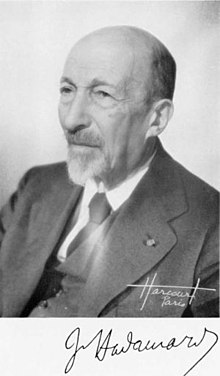
\includegraphics[width=0.5\marginparwidth]{Source/images/hadamard.jpg}
        \caption{ \scriptsize Jacques Salomon Hadamard (1865 - 1963) \cite{hadamard-wikipedia} fue un matemático francés. Trató temas de física matemática, colaboró en el establecimiento de las bases del análisis infinitesimal y desarrolló el teorema sobre el valor absoluto de un determinante.}
    \end{marginfigure}
    
    Como $E_{in}(w)$ es diferenciable podemos calcular los $w$ que minimizan  $E_{in}$.

    \begin{equation}
    \nabla E_{in}(w) = \frac{2}{N}(X^TXw - X^T y) =0
    \end{equation}
    Finalmente, para conseguir $\nabla  E_{in}(w) = 0$, buscamos $w$ cumpliendo que
    \begin{equation}
        X^TXw = X y
    \end{equation}

    Si $X^TX$ es invertible, $w = X^\dagger y$, donde $X^\dagger = (X^T X)^{-1}$ es la \textit{pseudo inversa} de $X$. El $w$ resultante es el único óptimo que minimiza $E_{in}$.  De lo contrario,  la pseudo inversa sí podría ser definida, pero la solución no sería única. \\
    
    En la práctica, $X^TX$ suele ser invertible porque $N$ es mucho mayo que $d+1$, así que habrá $d+1$ vectores linealmente independientes $x_n$.

    \subsection{El descenso de gradiente}
    
    \begin{marginfigure}
        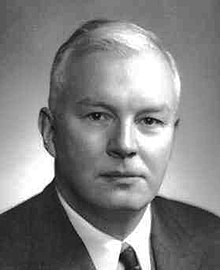
\includegraphics[width=0.5\marginparwidth]{Source/images/haskell.jpg}
        \caption{ \scriptsize Haskell Brooks Curry (1900-1982) \cite{haskell-wikipedia} fue un matemático y lógico estadounidense, especializado en teoría de sistemas y lógica combinatoria, fundamento de los lenguajes funcionales.}
    \end{marginfigure}
    
    El descenso de gradiente \cite{descenso-gradiente} \cite{gradient-descent-youtube} es uno de los algoritmos más populares para optimizar las redes neuronales. Su autoría se atribuye a Cauchy, quien fue el primero en sugerirlo en 1847. Hadamard propuso de forma independiente un método similar en 1907. La convergencia de este método para optimización de funciones no lineales fue estudiado por Haskell Curry en 1944. El método fue ampliamente estudiado y utilizado en las décadas posteriores \cite{gradient-descent-wikipedia}.
    
    \newpage\restoregeometry
    
    Este método consiste en minimizar una función objetivo $J(\theta)$ parametrizada por los parámetros $\theta \in \mathbb{R}^d$ de un modelo mediante la actualización de los parámetros en la dirección opuesta a la del gradiente de la función objetivo $\nabla_\theta J(\theta)$. La tasa de aprendizaje $\eta$ determina el número de pasos necesarios hasta alcanzar un mínimo local. \\
    
    Intuitivamente, seguimos la dirección de la pendiente de la superficie creada por la función objetivo (normalmente, el error cuadrático medio) hasta que alcanzamos un valle, dando pasos de una longitud determinada por $\eta$.
    
    \subsubsection{Variantes del Descenso de Gradiente}
    \paragraph{Descenso de Gradiente Batch \\}
    Calcula el gradiente de la función de coste con respeto a los parámetros $\theta$ para el conjunto de entrenamiento completo:
    \begin{equation}
        \theta = \theta - \eta \nabla_\theta J(\theta).
    \end{equation}
    Tiene un alto coste computacional y puede llegar a ser muy lento.
    
    \paragraph{Descenso de Gradiente Estocástico \\}
    Realiza la actualización de un parámetro para cada ejemplo de entrenamiento $x^{(i)}$ y etiqueta $y^{(i)}$.
    \begin{equation}
        \theta = \theta - \eta \nabla_\theta J (\theta; x^{(i)}; y^{(i)})
    \end{equation}
    
    \paragraph{Descenso de Gradiente Mini-Batch \\}
    Realiza una actualización para cada subconjunto de $n$ ejemplos de entrenamiento:
    \begin{equation}
        \theta = \theta - \eta \nabla_\theta J (\theta; x^{(i:i+n)}; y^{(i:i+n)})
    \end{equation}
    Con frecuencia se utiliza una combinación del método estocástico y mini Batch
    
    \subsection{Algoritmos de Descenso de Gradiente}
    Las variantes del descenso de gradiente presentadas se pueden refinar en algoritmos más eficientes, siguiendo su filosofía. \\
    
    Además, el valor que le demos a la tasa de aprendizaje $\eta$ es relevante. Cada algoritmo concreto le dará un valor, que puede ser constante o variable a conveniencia.
    \newpage
    
        \subsubsection{Momentum}
        El algoritmo Momentum está basado en el Descenso de Gradiente Estocástico. Intuitivamente, se basa en un pelota rodando cuesta abajo. Cuanto más rueda hacia una zona de menor altura, más rápido avanza. Esto lo aplicamos a la actualización de los parámetros: cuántas más actualizaciones de los parámetros que nos acercan a un mínimo local hacemos, más abruptas son.
        \begin{figure}[h]
            \center
            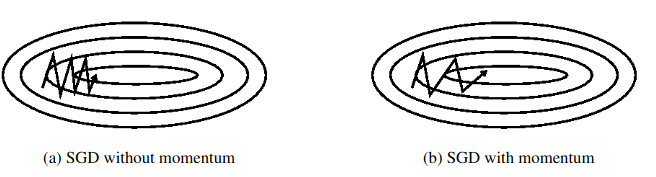
\includegraphics[width=\textwidth]{Source/images/momentum.png}
            \caption{Descenso de Gradiente Estocástico básico (izq) y algoritmo Momentum (dcha).}
        \end{figure}
        
        
\newpage\margenimagen
\section{Otras grandes figuras} 

\subsection{Geoffrey Hinton}

\begin{marginfigure}
    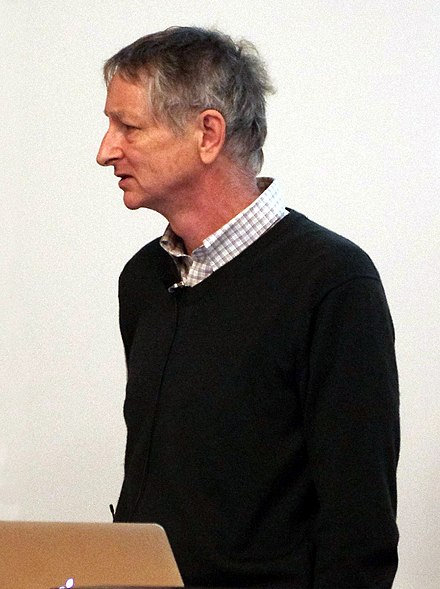
\includegraphics[width=\marginparwidth]{Source/images/Hinto_2013.jpg}
    \caption{Geoffey Hinton.}
\end{marginfigure}

Geoffrey Hinton (1947) es un psicólogo cognitivo e informático británico y canadiense \cite{geoffrey-hinton}. \\

En 1986 publicó junto a David Rumelhart y Ronald J. Williamsel el artículo que popularizaría el algoritmo de \textit{backpropagation} para redes neuronales multicapa \cite{rumelhart-hinton-williams}. \\

En 2018 se le concedió el premio Turing. \\

Actualmente trabaja a tiempo parcial en la universidad Toronto (Canadá) y en el equipo de investigación \textit{Google Brain}, un grupo de trabajo de Google dedicado al aprendizaje profundo y la creación y mejora de herramientas como TensorFlow y Google Translate, así como la mejora de imágenes y el aprendizaje de sistemas de encriptación simétrica usando redes generativas adversativas \cite{Google-Brain}.

\subsection{Yoshua Bengio}
\begin{marginfigure}
    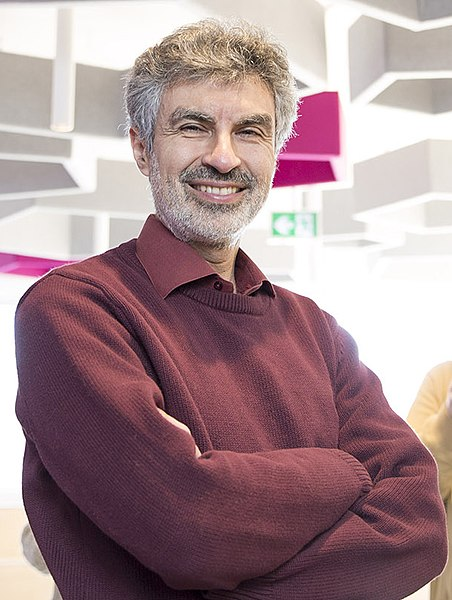
\includegraphics[width=\marginparwidth]{Source/images/Yoshua_Bengio.jpg}
    \caption{Yoshua Bengio.}
\end{marginfigure}

Yoshua Bengio \cite{bengio-wikipedia} es un informático canadiense que investiga sobre deep learning, traducción automática neural, redes generativas, auto encoders, modelos neurales del lenguaje y el meta aprendizaje. \\

Desde 2007 trabaja para Facebook aunque también es investigador en la universidad de Montréal y director del \textit{Montreal Institute for Learning Algorithms}. \\

En 2018 se le concedió el premio Turing. 

\newpage\restoregeometry
\section{Conclusiones}
El aprendizaje automático es un área de la informática joven, con una breve pero intensa historia. A pesar de basarse en conocimientos matemáticos sobradamente conocidos desde hace siglos, no ha sido hasta hace pocas décadas cuando se han puesto intensamente en práctica. \\

Al igual que el resto de disciplinas de la informática, su rápido desarrollo en un corto intervalo de tiempo ha supuesto una reinvención de la vida y relaciones humanas con respecto a tal y como las conocíamos. \\

Pocas ciencias han progresado tan velozmente como esta, tanto es así que la teoría matemática disponible empieza a no ser suficiente, lo que abre nuevas líneas de investigación. \\

Además, el gran impacto del aprendizaje automático en la sociedad ha repercutido también en la economía global. Ahora son las empresas tecnológicas las que lideran la economía y sus empleados, la nueva vanguardia científica. \\

Con la realización de este trabajo nos hemos acercado a los entresijos de este campo que desconocíamos y nos ha aportado una visión histórica más profunda del desarrollo de la ciencia.

\restoregeometry

%%%% TODO
%Muy interesante comentar que esta gente trabaja para empresas privadas tipo Facebook y Google. 

%TODO añadir ranking de quién publica más artículos de aprendizaje automático / visión por computador...

%%%%%%%%%%%%%%%%%%%%%%%%%%%%%%%%%%%%%% fin de secciones principales %%%%%%%%%%%
%COSAS IMPORTANTES: 
%- Comentar en el momento más oportuno que toda esta teoría comenzó a tener sentido cuando a nivel computacional eran asequibles, hasta el momento estuvieron aparcadas y sin hacerle mucho caso. 
%- Quizás fuera interesante añadir el pseudocódigo o imágenes aclarativas de qué se está haciendo. Para el perceptrón y tal podemos sacarlas de o los apuntes de aprendizaje automático o de mis trabajos. 
%- Dar ejemplo de cosillas que se desconocen actualmente: 

%Por ejemplo el teorema de aproximación se sabe que con una capa se aproxima, pero de manera empírica se sabe que aproxima mejor usando más capas ¿qué relación pues existe entre el número de capas ocultas y que converja más rápido?

%\newpage
%\section{Ejemplo de uso
%clasificando imágenes en Pytorch}
%TODO 
%No sabemos si incluirlo.


%%%%%%%%%%%%%%%%%%%%%%%%%%%%%%%%%%%%%%%%%%%%%%%%%%%%%%%%%%%%%%%%%%%%%%%%%%%%%%%
% BIBLIOGRAFÍA
\newpage

\printbibliography

\end{document}